
\section{Experimental Results}\label{sec:exp}

Here we present the results of our experiment conducted to measure the performance of the main parts of the system, the tokenizer and the matcher. First a description of the setup to run the benchmarks followed by a short explanation of the experiments and finally the results.

\mypar{Experimental Setup} The experiments were executed on an Intel Xeon Phi 7120 coprocessor. It consists of 61 cores and 16 GB of GDDR5 memory with a theoretical bandwidth of 352 GB/s. According to the documentation the Xeon Phi's optimal computational power can be reached running two threads per core, i.e. 120 threads.
For compilation the Intel Compiler version 15.0.0 20140723 was used with the following flags: \verb;-fopenmp; \verb;-std=c++11; \verb;-mmic; \verb;-Wall; \verb;-qopt-report3; \\ \verb;-qopt-report-phase=vec; \verb;-O3;.

The benchmarks focus on the tokenizer and the matcher. To generate test data, we used the XML benchmark project XMark \cite{Schmidt2002}. To measure the scalability of the tokenizer 100 test runs were conducted. For each run, an input file of the size of 2 GB was used which contained 61'113'640 tokens. First, we measured the performance of the tokenizer working with 1 thread. Then we increased the number of threads to 2, 4, 8, 16, 32, 60, 120, 180 and 240. Each experiment was run ten times. The results were built with the average of these runs. Similarly, the matcher was tested with files of the sizes 2 GB (27'620'104 tokens), 4 GB (55'236'244 tokens) and 8 GB (110'467'124 tokens). For each file 10 different experiments were run. The first experiment matched 1 query, i.e. running with 1 thread, the second matched 2 queries and the following experiments matched 4, 8, 16, 32, 60, 120, 180 and 240 queries. Again, the result is the average of the runs.

\mypar{Results}
The experiments reveal clearly, that the throughput of the tokenizer increases with the number of threads. In figure ~\ref{tokenizer_throughput}, where the throughput against the number of threads is plotted, nearly linear scaling can be observed. While the benefits of more threads are significant up to 120 threads, i.e. two threads per core, less performance can be gained from 120 up to 240 threads. These results confirm the optimal use of processors, which is at two threads per core, as we mentioned earlier.

\begin{figure}[h]\centering
  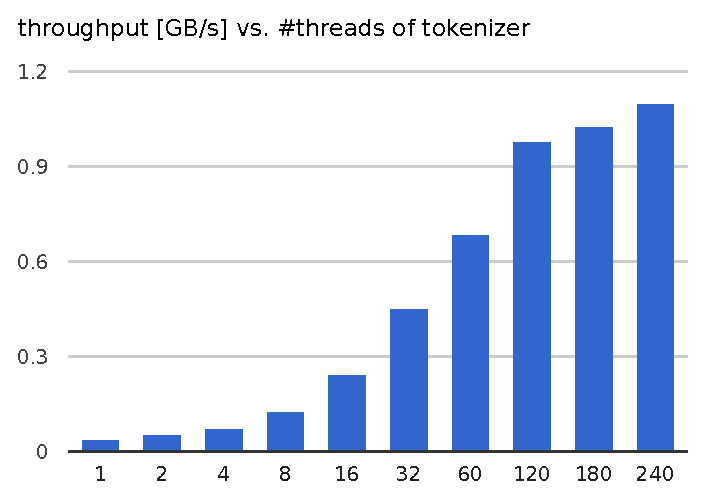
\includegraphics[scale=.66]{img/tokenizer_throughput_2.eps}
  \caption{Throughput of the tokenizer in GB/s measured with different numbers of threads.
  \label{tokenizer_throughput}}
\end{figure}

In figure~\ref{matcher_throughput} the throughput of the matcher against the numbers of queries, i.e. threads, is plotted. Since the file size alone does not reveal enough information about the complexity, or the number of tokens in the XML data, the throughput is given in the number of tokens that are processed per second. Until up to 60 queries there is no significant drop of the performance, while with 120 queries and more the throughput plummets. Weak scaling is observable for up to 60 threads. When the number of threads exceeds the number of cores the performance suffers. The sudden decrease of performance for 8 GB might be due to the memory access pattern on the Xeon Phi, which becomes apparent, when more threads operate at the same time on larger amount of data. Pursuing experiments that confirm this hypothesis would exceed the format of this report. 

\begin{figure}[h]\centering
  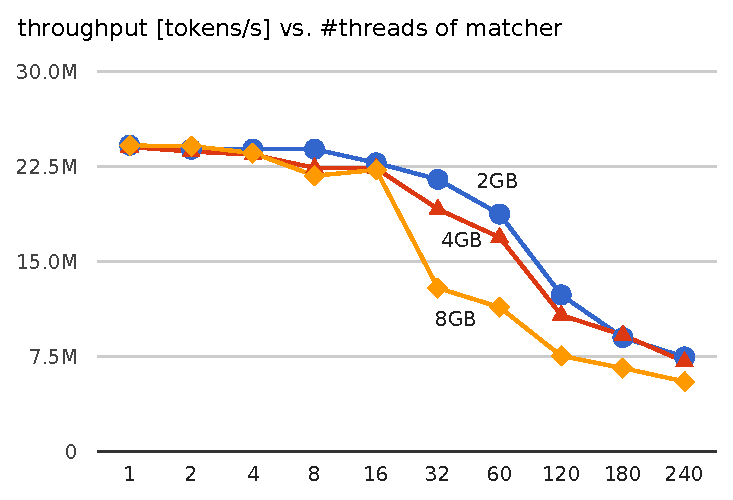
\includegraphics[scale=.66]{img/matcher_throughput_2.eps}
  \caption{Throughput of the matcher in tokens/s comparing different input sizes. \label{matcher_throughput}}
\end{figure}

A direct comparison of the processing time of the tokenizer and the matcher is plotted in figure ~\ref{matcher_tokenizer_pt}. The numbers represent the absolute processing time of a XML file of 2 GB. One can see, that the processing time of the matcher stays practically the same, even when increasing the numbers of queries being processed, while decreasing drastically for the tokenizer when more threads are provided.

\begin{figure}[h]\centering
  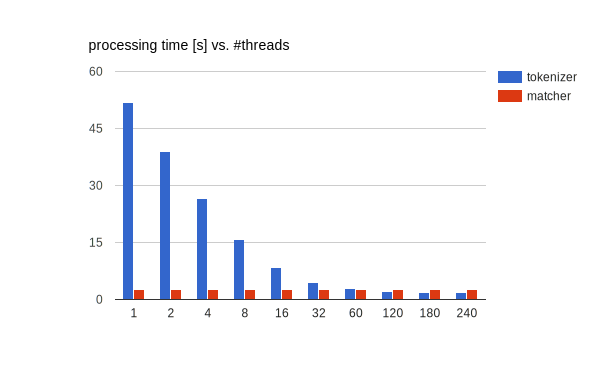
\includegraphics[scale=.66]{img/matcher_tokenizer_p_time.eps}
  \caption{Processing time of matcher and tokenizer in comparison for an input of size 2 GB.
  \label{matcher_tokenizer_pt}}
\end{figure}

The total throughput of the tokenizer and matcher running with 120 threads is 0.29 GB/s.
\todo{Exact Data / Experiment basis for 0.29GB/s value?}